\documentclass{beamer}	
\usecolortheme{default}

\setbeamertemplate{caption}{\raggedright\insertcaption\par}

\usepackage{tabularx}
\usepackage{booktabs}
\usepackage{multirow}
\newcolumntype{C}{>{\centering\arraybackslash}X}
\usepackage{proof}
\usepackage{amsmath}
\usepackage{wasysym}
\usepackage{tikz}
\usetikzlibrary{arrows.meta,positioning,matrix}
\usetikzlibrary{shapes.multipart, calc}
\usepackage{tikz-qtree}

\newcommand{\term}[1]{\ensuremath{\mathtt{#1}}}
\newcommand{\li}{\!\multimap\!}
\newcommand{\lotimes}{\!\otimes\!}
\newcommand{\loplus}{\!\oplus\!}
\newcommand{\lin}[1]{\langle#1\rangle}
\newcommand{\lint}[1]{[#1]}
\newcommand{\cat}[1]{\footnotesize \textsc{#1}}	
\newcommand{\W}[1]{\scriptsize #1}
\newcommand{\etext}[1]{\scriptsize {\textit{#1}}}
\newcommand{\smain}{\cat{S}$_{\text{main}}$}
\newcommand{\ssub}{\cat{S}$_{\text{sub}}$}
\newcommand{\type}[2]{\scriptsize\ensuremath{\textcolor{#2}{#1}}}
\newcommand{\red}[1]{\textcolor{red}{{}_#1}}

\title{Type \& Proof Extraction}
\author{K. Kogkalidis}
\institute{Logic \& Language 2020}

\begin{document}

\begin{frame}
\centering
\includegraphics[width=0.85\textwidth]{andnow.jpg}
\end{frame}

\begin{frame}{The State of Affairs}
\small
\begin{block}{NLP in the last decade}
	Over-parameterized data-intensive unsupervised models\\
	\begin{tabularx}{0.5\textwidth}{ll}
	2008-2013 & Compressed co-occurrence vectors, $n$-grams\\
	2013-2016 & ``\textit{word2vec}'' era: neural vectors\\
	2016-2018 & \textit{rnn} based language models (ELMo)\\
	2018-2020 & \textit{transformer} based language models (GPT-2, BERT, \dots)
	\end{tabularx}
\end{block}
\vfill

\pause
\begin{flushright}
	..where is syntax?
\end{flushright}

\end{frame}

\begin{frame}{Towards Type-Driven \& Neural Textual Representations}
\small
The agenda:
\begin{itemize}
	\item[$\lambda$] \alt<2->{\alert{Choosing the logic}}{Choosing the logic}
	\item[$\lambda$] \alt<2->{\alert{Making a dataset: proofs and lexical type assignments}}{Making a dataset: proofs and lexical type assignments}
	\item[$\lambda$] \alt<2->{\textcolor{gray}{Learning the type assignment process}}{Learning the type assignment process}
	\item[$\lambda$] \alt<2->{\textcolor{gray}{Navigating the proof space}}{Navigating the proof space}
	\item[$\lambda$] \alt<2->{\textcolor{gray}{Syntax-aware \& type-correct text representations}}{Syntax-aware \& type-correct text representations}
\end{itemize}
\end{frame}

\begin{frame}{Syntax-Semantics Interface}
	% tlg : syntax -> der -> sem
	% acg: 	tecto	-> pheno
	%				-> sem
	% now:	pheno	-> syntax	-> der	-> sem
	% 		we leave the pointwise translation from pheno to syntax implicit, avoiding the trap of ACG exploding lexicon
	%		parse instead directly on tectogrammatic form
	%		the lambda terms obtained are the same as doing pheno -> tecto (.) parse (.) tecto-> pheno 

	\alt<3->{
		\centering
		Now
		\vspace{5pt}
		
		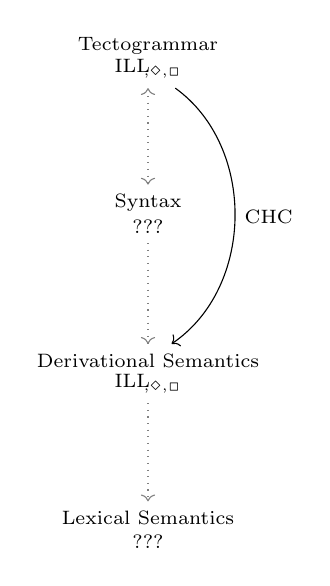
\begin{tikzpicture}
			\node (abstract)	at	(0, 0) 		{\scriptsize Tectogrammar};
			\node (depill)	at	(0, -0.3)	{\scriptsize ILL$_{\li, \Diamond, \Box}$};
			\node (syntax)	at 	(0, -2)		{\scriptsize Syntax};
			\node (depnl)	at 	(0,	-2.3)	{\scriptsize ???};
			\node (der)		at	(0, -4)		{\scriptsize Derivational Semantics};
			\node (derill)	at 	(0, -4.3)	{\scriptsize ILL$_{\li, \Diamond, \Box}$};
			\node (sem)		at 	(0, -6)		{\scriptsize Lexical Semantics};
			\node (seml)		at	(0, -6.3)	{\scriptsize ???}; 
			
			\draw (depill) edge[bend left=55, ->] node[right] {\scriptsize CHC} (der);
			\draw (depill) 	edge[<->, gray, dotted] (syntax);
			\draw (depnl)	edge[->, gray, dotted] (der); 
			\draw (derill) 	edge[->, gray, dotted] (sem);
		\end{tikzpicture}
	}{
		\begin{minipage}[t]{0.5\textwidth}
			\centering Type-logical perspective
			\vspace{5pt}
			
			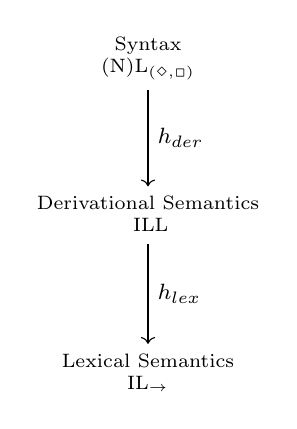
\begin{tikzpicture}
				\node (syntax) at (0,0) {\scriptsize Syntax};	
				\node (nl) at (0,-0.3) {\scriptsize (N)L$_{(\Diamond, \Box)}$};
				\node (der) at (0,-2) {\scriptsize Derivational Semantics};
				\node (mill) at (0,-2.3) {\scriptsize ILL$_{\li}$};
				\node (sem) at (0,-4) {\scriptsize Lexical Semantics};
				\node (il) at (0, -4.3) {\scriptsize IL$_{\to}$};
		
				\draw (nl) edge[->] node[midway, right] {\footnotesize $h_{der}$} (der);
				\draw (mill) edge[->] node[midway, right] {\footnotesize $h_{lex}$} (sem);
			\end{tikzpicture}		
			\end{minipage}%
			\pause
			\begin{minipage}[t]{0.5\textwidth}
					\centering ACG perspective
					\vspace{5pt}
					
			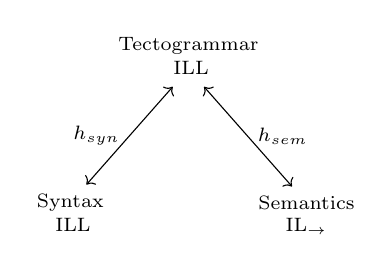
\begin{tikzpicture}		
				\node (abstract) 	at 	(0, 0) 		{\scriptsize Tectogrammar};
				\node (amill)		at	(0, -0.3)	{\scriptsize ILL$_{\li}$};
				\node (syntax)		at	(-1.5, -2) 	{\scriptsize Syntax};
				\node (symill) 		at	(-1.5, -2.3)	{\scriptsize ILL$_{\li}$};
				\node (semantics)	at 	(1.5, -2) 	{\scriptsize Semantics};
				\node (semill)		at	(1.5, -2.3)	{\scriptsize IL$_{\to}$};
				\draw (amill) edge[<->] node[midway, left] {\scriptsize $h_{syn}$} (syntax);
				\draw (amill) edge[<->] node[midway, right] {\scriptsize $h_{sem}$} (semantics);
			\end{tikzpicture}		
		\end{minipage}
	}
\end{frame}

\begin{frame}{Abstract syntax with NLP}
\small
\alt<2->{
	Lexicon $\mathcal{L}$ assigning words types from: $\visible<3->{A \ 
							\visible<4->{ | \ \Diamond^d T \li T' \ 
							\visible<5->{ | \ \Box^d \left( T \li T\right) }}}$
	
	\vfill

	\begin{minipage}[t]{0.9\textwidth}
		\begin{tabularx}{0.9\textwidth}{rlcrl}
		\visible<3->{I, animals, ducks & : $np$} & & \visible<4->{fly, swim & : $\Diamond^{su}np \li s$}\\
		\visible<4->{like & : $\Diamond^{obj}np \li \Diamond^{su}np \li s$} & & \visible<5->{gracefully & : $\Box^{mod}\left(s \li s \right)$}\\
		\visible<6->{that & \multicolumn{4}{l}{: $\Diamond^{body}\left(\Diamond^{su} np \li s\right) \li \Box^{mod}\left(np\li np \right)$}}\\
		\end{tabularx}
	\end{minipage}		

	\begin{minipage}{0.99\textwidth}		
		\scriptsize
		\centering
		\alt<3>{
			\[
				\infer[\mathcal{L}]{\term{ducks}: np}{\text{ducks}}
			\]}
		{
		\alt<4>{
			\[
				\infer[\li E]{\langle \text{ducks} \rangle^{su} \  \text{fly} \vdash  s}{
					\infer[\mathcal{L}]{\Diamond^{su}np \li s}{\text{fly}}
					&
					\infer[\Diamond^{su} I]{\langle \text{ducks} \rangle^{su} \vdash \Diamond^{su} np}{
						\infer[\mathcal{L}]{np}{\text{ducks}}
					}
				}
			\]
			\[
				\term{fly\ (ducks)^{su}}
			\]
		}{
		\alt<5>{
			\[
				\infer[\li E]{\langle \text{ducks} \rangle^{su} \ \text{fly} \ \langle \text{gracefully} \rangle^{mod} 
				\vdash  s}{
					\infer[\Box^{mod} E]{\langle \text{gracefully} \rangle^{mod} \vdash s \li s }{
						\infer[\mathcal{L}]{\Box^{mod} \left( s \li s \right)}{\text{gracefully}}
					}
					&
					\infer{\langle \text{ducks} \rangle^{su} \  \text{fly} \vdash s}{
						\infer*{}{}
					}
				}
			\]
			\[
				\term{(gracefully)_{mod}\ (\term{fly}\ (ducks)^{su})}
			\]
		}{
		\alt<6>{
			\scriptsize
			\[
				\infer[\li E]{\text{animals}\ \langle \text{that}\ \langle \text{swim}\rangle^{body}\rangle^{mod} \vdash np}{
					\infer[\mathcal{L}]{np}{\text{animals}}
					&
					\hspace{-20pt}
					\infer[\Box^{mod} E]{\langle \text{that}\ \langle \text{swim}\rangle^{su}\rangle^{mod}\vdash np \li np}{
						\infer[\li E]{\text{that}\ \langle \text{swim}\rangle^{su} \vdash \Box^{mod} (np \li np)}{
							\infer[\mathcal{L}]{\Diamond^{body}\left(\Diamond^{su} np \li s\right) \li \Box^{mod}\left(np\li np \right)}{\text{that}}
							&
							\infer[\Diamond^{body} I]{\langle \text{swim}\rangle^{body} \vdash \Diamond^{body}\left(\Diamond^{su} np \li s \right)}{
								\infer[\mathcal{L}]{\Diamond^{su}np\li s}{\text{swim}}
							}
						}
					}
				}
			\]
			\[
				\term{\left( that\ {(swim)}^{body} \right)_{mod}\ animals}
			\]
		}}}}{}
	\end{minipage}

	
}{
	\begin{block}{Grammar}
		ILL$_{\li}$ plus $\Diamond, \Box$ modalities for \textit{dependency domain demarkation}.
	\end{block}
	\vfill
		
	Types inductively defined by:
	\[
		\mathcal{T} := A \ | \  T \li T' \ | \ \Diamond^d  T \ | \ \Box^d T \qquad A \in \mathcal{A}, T \in \mathcal{T}
	\]
	\vfill	
	
	Rules:
	\begin{align*}
		\infer[\li E]{\Gamma, \Delta \vdash \term{f\ x}: B}{\Gamma \vdash \term{f}: A \li B & \Delta \vdash \term{x}: A}
		&\qquad
		\infer[\li I]{\Gamma \vdash \term{\lambda x.y}: A \li B}{\Gamma, \term{x}: A \vdash \term{y}: B} \\
		\infer[\Diamond^d I]{\langle \Gamma \rangle^{d} \vdash \term{x^d}: \Diamond^d A}{\Gamma \vdash \term{x}: A}
		&\qquad
		\infer[\Box^d E]{\langle \Gamma \rangle^{d} \vdash \term{x_d}: A}{\Gamma \vdash \term{x}: \Box^d A}
	\end{align*}
}
\end{frame}

\begin{frame}{Why ILL$_{\li, \Diamond, \Box}$?}
\small
\begin{block}{Why ILL$_{\li}$?}
	\begin{itemize}
	\item Easier to extract from corpora
	\item Massive reduction in lexical ambiguity 
	\item Abstract away from trivial word-order permutations
	\item Surface syntax matters little to semantics
	\end{itemize}
\end{block}
\begin{block}{Why $\Diamond, \raisebox{1.5pt}{\ensuremath{\Box}}$?}
	\begin{itemize}
	\item Easier to interpret
	\item Subsume dependency parsing
	\item More informative for semantics 
	\item Modalities can regulate non-logical parsing
	\end{itemize}
\end{block}

\end{frame}

\begin{frame}{From parse graphs to ILL$_{\li, \Diamond, \Box}$ types}
	\small
	\begin{block}{algorithm: graph flooding on dags}
		init with maps
		\begin{itemize}
			\item[-] from pos \& phrasal categories to $\mathcal{A}$	\\
			\quad e.g. $\textsc{np} \to np,\ \textsc{inf} \to inf, \dots$
			\item[-] from grammatical roles to $\Diamond$ (complements) and $\Box$ (adjuncts)\\
			\quad e.g. $su \to \Diamond^{su}, obj \to \Diamond^{obj}, \dots, mod \to \Box^{mod}, det \to \Box^{det}$
		\end{itemize}
		and a strict total order over $\Diamond$, \\
		e.g. $\Diamond^{su} > \Diamond^{obj}$
	\end{block}
\end{frame}

\begin{frame}{Simple case: trees}
	\small
	\begin{minipage}{0.5\textwidth}
	\centering
	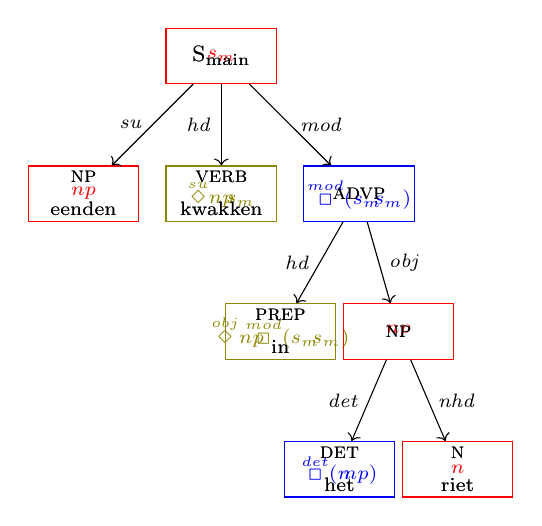
\begin{tikzpicture}[
	every text node part/.style={align=center},
	every node/.style={transform shape},
	block/.style={rectangle, inner sep=0pt, minimum width=40pt, minimum height=20pt},
	rblck/.style={rectangle, draw=red, inner sep=0pt, minimum width=40pt, minimum height=20pt},
	bblck/.style={rectangle, draw=blue, inner sep=0pt, minimum width=40pt, minimum height=20pt},
	oblck/.style={rectangle, draw=olive, inner sep=0pt, minimum width=40pt, minimum height=20pt}	
	]
	
	\alt<3->{
	\node[block] (smain) 	at (0, 0) 			{\type{s_m}{red}};}{
	\alt<2>{
	\node[rblck] (smain) 	at (0, 0) 			{\smain};}{
	\node[block] (smain) 	at (0, 0) 			{\smain};}}
	
	\alt<3->{
	\node[block] (eenden) 	at (-1.75, -1.75)		{\type{np}{red}};}{
	\alt<2>{
	\node[rblck] (eenden) 	at (-1.75, -1.75)		{\cat{np}\\ \W{eenden}};}{
	\node[block] (eenden) 	at (-1.75, -1.75)		{\cat{np}\\ \W{eenden}};}}

	\alt<7->{
	\node[block] (kwakken) 	at (0, -1.75) 		{\type{\overset{su}{\Diamond}np \li s_m}{olive}};}{
	\alt<6>{	
	\node[oblck] (kwakken) 	at (0, -1.75) 		{\cat{verb}\\ \W{kwakken}};}{
	\node[block] (kwakken) 	at (0, -1.75) 		{\cat{verb}\\ \W{kwakken}};}}
	
	
	\alt<5->{
	\node[block] (ihr)		at (1.75, -1.75) 		{\type{\overset{mod}{\Box}(s_m\li s_m)}{blue}};}{
	\alt<4>{
	\node[bblck] (ihr)		at (1.75, -1.75) 		{\cat{advp}};}{
	\node[block] (ihr)		at (1.75, -1.75) 		{\cat{advp}};}}
	
	\alt<7->{
	\node[block] (in)		at (0.75, -3.5) 		{\type{\overset{obj}{\Diamond}np\!\li\!\!\overset{mod}{\Box}(s_m\li s_m) }{olive}};}{
	\alt<6>{
	\node[oblck] (in)		at (0.75, -3.5) 		{\cat{prep}\\ \W{in}};}{
	\node[block] (in)		at (0.75, -3.5) 		{\cat{prep}\\ \W{in}};}}
	
	\alt<3->{
	\node[block] (hr)		at (2.25, -3.5) 		{\type{np}{red}};}{
	\alt<2>{
	\node[rblck] (hr)		at (2.25, -3.5) 		{\cat{np}};}{
	\node[block] (hr)		at (2.25, -3.5) 		{\cat{np}};}}
	
	\alt<5->{
	\node[block] (h)			at (1.5, -5.25) 		{\type{\overset{det}{\Box}(n\li np)}{blue}};}{
	\alt<4>{
	\node[bblck] (h)			at (1.5, -5.25) 		{\cat{det}\\ \W{het}};}{
	\node[block] (h)			at (1.5, -5.25) 		{\cat{det}\\ \W{het}};}}
	
	\alt<3->{
	\node[block] (r)			at (3, -5.25) 		{\type{n}{red}};}{
	\alt<2>{
	\node[rblck] (r)			at (3, -5.25) 		{\cat{n}\\ \W{riet}};}{
	\node[block] (r)			at (3, -5.25) 		{\cat{n}\\ \W{riet}};}}
	
	\draw (smain) 	edge[->]		node[left] 	{\etext{su}} 	(eenden);
	\draw (smain) 	edge[->]		node[left] 	{\etext{hd}} 	(kwakken);
	\draw (smain) 	edge[->]		node[right] {\etext{mod}} 	(ihr);
	
	\draw (ihr)	 	edge[->]		node[left] 	{\etext{hd}} 		(in);
	\draw (ihr)	 	edge[->]		node[right] {\etext{obj}} 		(hr);
	
	\draw(hr)		edge[->]		node[left] 	{\etext{det}}		(h);
	\draw(hr)		edge[->]		node[right] {\etext{nhd}}		(r);
	\end{tikzpicture}\vfill
	
	``eenden kwakken in het riet''
	\end{minipage}%
	\scriptsize
	\begin{minipage}{0.5\textwidth}
	while graph not fully typed, do:
	\begin{itemize}
		\visible<2->{
		\item assign \textcolor{red}{stand-alone nodes}	\\
				\quad no incoming adjunct or head edge\\
				\visible<3->{\quad \textbf{type} via the $\mathcal{A}$-map}}
		\visible<4->{
		\item assign \textcolor{blue}{adjuncts}\\
				\quad incoming adjunct edge\\
				\quad parent is typed\\
				\visible<5->{\quad \textbf{type}\\
				\quad if mod: boxed endofunctor of parent\\
				\quad else:from comp sibs to parent}}
		\visible<6->{
		\item assign \textcolor{olive}{heads} \\
				\quad incoming head edge\\
				\quad parent is typed\\
				\quad no untyped complement sibs\\
				\visible<7->{\quad \textbf{type} from comp sibs to parent}}
	\end{itemize}
	\vfill
	\end{minipage}
\end{frame}

\begin{frame}{Harder case: unbounded dependencies}
	\small
	\begin{minipage}{0.5\textwidth}
	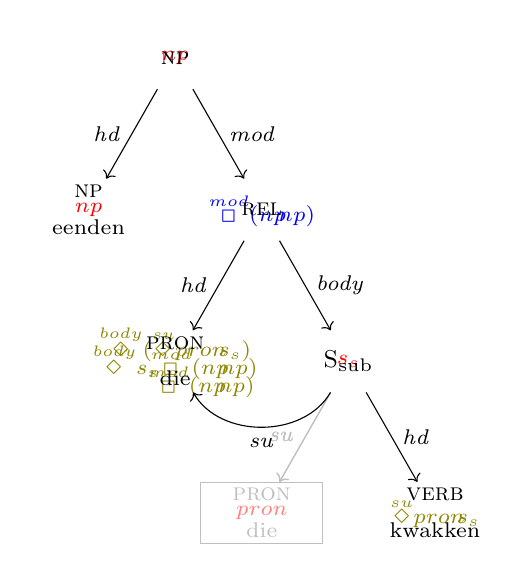
\begin{tikzpicture}[
	every text node part/.style={align=center},
	scale=1.1,
	every node/.style={transform shape},
	block/.style={rectangle, inner sep=0pt, minimum width=40pt, minimum height=20pt},
	rblck/.style={rectangle, draw=red, inner sep=0pt, minimum width=40pt, minimum height=20pt},
	bblck/.style={rectangle, draw=blue, inner sep=0pt, minimum width=40pt, minimum height=20pt},
	oblck/.style={rectangle, draw=olive, inner sep=0pt, minimum width=40pt, minimum height=20pt}	
	]
	
	\alt<3->{
	\node[block]		at (0, 0)			(root)		{\type{np}{red}};}{
	\node[block]		at (0, 0)			(root)		{\cat{np}};}
	
	\alt<3->{
	\node[block]		at (-1, -1.75)		(eenden)		{\type{np}{red}};}{
	\node[block]		at (-1, -1.75)		(eenden)		{\cat{np}\\ \W{eenden}};}
	
	\alt<3->{
	\node[block]		at (1, -1.75)		(dk)			{\type{\overset{mod}{\Box}(np \li np)}{blue}};}{
	\node[block]		at (1, -1.75)		(dk)			{\cat{rel}};}
	
	\alt<4->{
	\node[block]		at (0, -3.5)			(die)		
		{\type{\overset{body}{\Diamond}(\overset{su}{\Diamond}pron \li s_s)}{olive}\\
		\qquad \type{\li \overset{mod}{\Box}(np \li np)}{olive}};}{
	\alt<3->{
	\node[block]		at (0, -3.5)			(die)		{\type{\overset{body}{\Diamond}s_s \li \overset{mod}{\Box}(np \li np)}{olive}};}{
	\node[block]		at (0, -3.5)			(die)		{\cat{pron}\\ \W{die}};}}
	
	\alt<3->{
	\node[block]		at (2, -3.5)			(ssub)		{\type{s_{s}}{red}};}{
	\node[block]		at (2, -3.5)			(ssub)		{\ssub};}
	
	\alt<3->{
	\node[block]		at (3, -5.25)		(kwakken)	{\type{\overset{su}{\Diamond}pron \li s_s}{olive}};}{
	\node[block]		at (3, -5.25)		(kwakken)	{\cat{verb}\\ \W{kwakken}};}	
	
	\draw (root)		edge[->]		node[left] 	{\etext{hd}}		(eenden);	
	\draw (root)		edge[->]		node[right] {\etext{mod}}	(dk);
	\draw (dk)		edge[->]		node[left] 	{\etext{hd}}		(die);
	\draw (dk)		edge[->]		node[right] 	{\etext{body}}	(ssub);
	\draw (ssub)		edge[->]		node[right] 	{\etext{hd}}		(kwakken);	
	

	\alt<3->{
	\node[block]		at (1, -5.25)		(copy)	{\type{pron}{red!50}};
	\draw (ssub)		edge[->,draw=gray!50] node[left] {\textcolor{gray!50}{\etext{su}}}		(copy);
	}{
	\alt<2->{
	\node[block,draw=gray!50]		at (1, -5.25)		(copy)	{\textcolor{gray!50}{\cat{pron}}\\ \W{\textcolor{gray!50}{die}}};
	\draw (ssub)		edge[->,draw=gray!50] node[left] {\textcolor{gray!50}{\etext{su}}}		(copy);}{
	\draw (ssub)		edge[->, bend left=60] node[below] {\etext{su}}		(die);}}
	\end{tikzpicture}
	
	\begin{center}
		``eenden die kwakken''
	\end{center}	
	\end{minipage}%
	\begin{minipage}{0.5\textwidth}
	\scriptsize
	\begin{itemize}
	\visible<2->{
	\item 	detach non-local dependencies}
	\visible<3->{
	\item 	type trees as before}
	\visible<4->{
	\item	redact ghosts types from comp sibs}
	\end{itemize}
	\vfill
	\end{minipage}
\end{frame}

\begin{frame}{\alt<5>{ACG Flashback}{Hardest case: Ellipses}}
	\small
	
	\alt<5>{
	\begin{center}
		\vspace{5pt}
		\includegraphics[width=0.8\textwidth]{vietnam.jpg}
	\end{center}
	
	\footnotesize
	\begin{itemize}
		\item 	each conjunct represents a tuple of types \\
				$c = (t_1, t_2, \dots t_n) \equiv t_1 \lotimes t_2 \lotimes \dots \lotimes t_n$
		\item  encoded as the higher-order function $(c \li r)\li r$ and curried into 
		$(t_1 \li t_2 \li \dots \li t_n \li r)\li r$
	\end{itemize}
	}{
	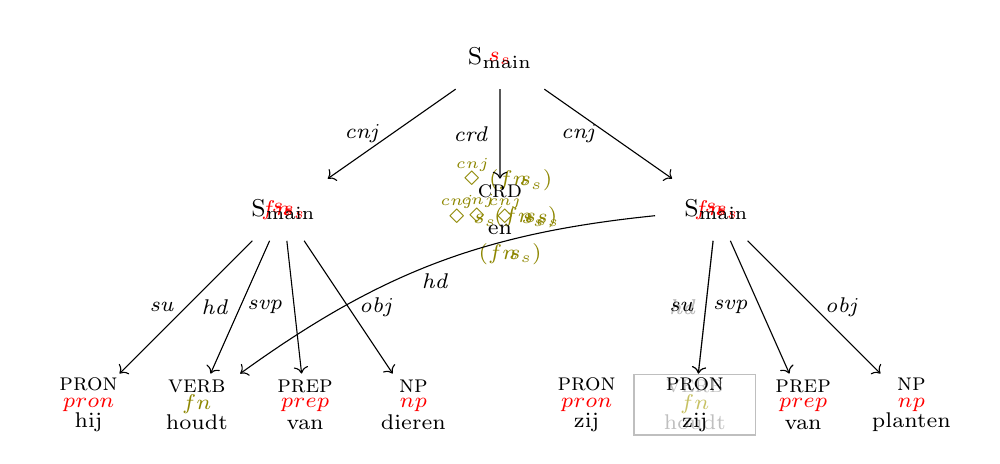
\begin{tikzpicture}[
	every text node part/.style={align=center},
	scale=1.1,
	every node/.style={transform shape},
	block/.style={rectangle, inner sep=0pt, minimum width=40pt, minimum height=20pt},
	rblck/.style={rectangle, draw=red, inner sep=0pt, minimum width=40pt, minimum height=20pt},
	bblck/.style={rectangle, draw=blue, inner sep=0pt, minimum width=40pt, minimum height=20pt},
	oblck/.style={rectangle, draw=olive, inner sep=0pt, minimum width=40pt, minimum height=20pt}	
	]
	\alt<3->{
	\node[block]			at (0, 0)			(root)		{\type{s_s}{red}};
	}{
	\node[block]			at (0, 0)			(root)		{\smain};}
	
	\alt<3->{
	\alt<4->{
	\node[block]			at (-2.5, -1.75)	(s1)				{\type{fn \li s_s}{red}};
	\node[block]			at (2.5, -1.75)		(s2)			{\type{fn \li s_s}{red}};
	}{
	\node[block]			at (-2.5, -1.75)	(s1)			{\type{s_s}{red}};
	\node[block]			at (2.5, -1.75)		(s2)			{\type{s_s}{red}};}
	\alt<6->{
	\node[block]			at (0, -1.75)		(en)			{
		\type{\overset{cnj}{\Diamond}(fn\li s_s)\li}{olive}\\
		~\type{\overset{cnj}{\Diamond}(fn\li s_s)\li}{olive}\\
		~~\type{(fn\li s_s)}{olive}};}{
	\node[block]			at (0, -1.75)		(en)			{\type{\overset{cnj}{\Diamond}s_s \li 
	\overset{cnj}{\Diamond}s_s \li s_s}{olive}};}}{
	\node[block]			at (-2.5, -1.75)	(s1)			{\smain};
	\node[block]			at (2.5, -1.75)		(s2)			{\smain};
	\node[block]			at (0, -1.75)		(en)			{\cat{crd}\\ \W{en}};}	
	
	\alt<3->{
	\node[block]			at (-4.75, -4)			(hij)		{\type{pron}{red}};
	\node[block]			at (-3.5, -4)			(houdt)		{\type{fn}{olive}};
	\node[block]			at (-2.25, -4)			(van)		{\type{prep}{red}};
	\node[block]			at (-1, -4)			(dieren)		{\type{np}{red}};}{
	\node[block]			at (-4.75, -4)			(hij)		{\cat{pron}\\ \W{hij}};
	\node[block]			at (-3.5, -4)			(houdt)		{\cat{verb}\\ \W{houdt}};
	\node[block]			at (-2.25, -4)			(van)		{\cat{prep}\\ \W{van}};
	\node[block]			at (-1, -4)			(dieren)		{\cat{np}\\ \W{dieren}};}

	\alt<3->{
	\node[block]			at (1, -4)			(zij)		{\type{pron}{red}};
	\node[block]			at (2.25, -4)		(houdt2)		{\type{fn}{olive!50}};
	\draw (s2)			edge[->,color=gray!50] node[left]	{\etext{\textcolor{gray!50}{hd}}} (houdt2);
	}{
	\alt<2->{
	\node[block]			at (1, -4)			(zij)		{\cat{pron}\\ \W{zij}};
	\node[block,draw=gray!50]			at (2.25, -4)			(houdt2)		{\cat{\textcolor{gray!50}{verb}}\\ \W{\textcolor{gray!50}{houdt}}};
	\draw (s2)			edge[->,color=gray!50] node[left]	{\etext{\textcolor{gray!50}{hd}}} (houdt2);}{
	\node[block]			at (2.25, -4)			(zij)		{\cat{pron}\\ \W{zij}};
	\draw (s2)			edge[->, bend right=15]			node[midway, below]			{\etext{hd}}			(houdt);	}}
	
	\alt<3->{
	\node[block]			at (3.5, -4)			(van2)			{\type{prep}{red}};
	\node[block]			at (4.75, -4)		(planten)		{\type{np}{red}};}{
	\node[block]			at (3.5, -4)			(van2)			{\cat{prep}\\ \W{van}};
	\node[block]			at (4.75, -4)		(planten)		{\cat{np}\\ \W{planten}};}

	\draw (root)			edge[->]			node[left]	{\etext{crd}}		(en);
	\draw (root)			edge[->]			node[left]	{\etext{cnj}}		(s1);
	\draw (root)			edge[->]			node[left]	{\etext{cnj}}		(s2);
	
	\draw (s1)			edge[->]			node[left]	{\etext{su}}			(hij);	
	\draw (s1)			edge[->]			node[left]	{\etext{hd}}			(houdt);	
	\draw (s1)			edge[->]			node[left]	{\etext{svp}}		(van);	
	\draw (s1)			edge[->]			node[right]	{\etext{obj}}		(dieren);	

	\draw (s2)			edge[->]			node[left]	{\etext{su}}			(zij);	
	\draw (s2)			edge[->]			node[left]	{\etext{svp}}			(van2);	
	\draw (s2)			edge[->]			node[right]	{\etext{obj}}		(planten);	
	\end{tikzpicture}
	\begin{center}
		``hij houdt van dieren en zij van planten''
	\end{center}
	
	\begin{minipage}{0.58\textwidth}
	\scriptsize
	\begin{itemize}
	\visible<2->{
	\item 	detach and type trees as usual}
	\visible<4->{
	\item 	redact missing types from \textbf{both} conjuncts}
	\visible<5->{
	\item update coord type \& attach copies at top level}
	\end{itemize}
	\end{minipage}%
	\begin{minipage}{0.42\textwidth}
	\scriptsize
	\begin{flushright}
		\visible<3->{
		$fn := \overset{svp}{\Diamond}prep \li \overset{obj}{\Diamond}{np}\li \overset{su}{\Diamond}pron \li s_s$}
	\end{flushright}
	\end{minipage}
	}
\end{frame}

\begin{frame}{Hardest case: Ellipses}
	\small
	
	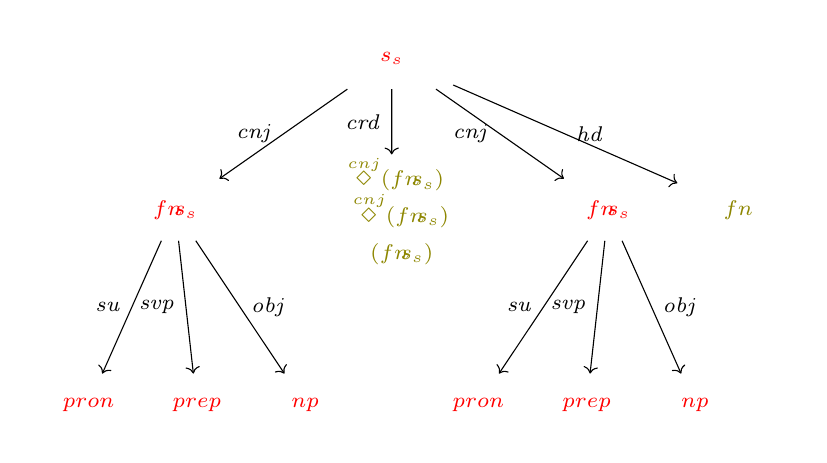
\begin{tikzpicture}[
	every text node part/.style={align=center},
	scale=1.1,
	every node/.style={transform shape},
	block/.style={rectangle, inner sep=0pt, minimum width=40pt, minimum height=20pt},
	rblck/.style={rectangle, draw=red, inner sep=0pt, minimum width=40pt, minimum height=20pt},
	bblck/.style={rectangle, draw=blue, inner sep=0pt, minimum width=40pt, minimum height=20pt},
	oblck/.style={rectangle, draw=olive, inner sep=0pt, minimum width=40pt, minimum height=20pt}	
	]
	\node[block]			at (0, 0)			(root)		{\type{s_s}{red}};
	\node[block, outer sep=0pt]			at (4, -1.75)		(houdt)		{\type{fn}{olive}};
		
	\node[block]			at (-2.5, -1.75)	(s1)				{\type{fn \li s_s}{red}};
	\node[block]			at (2.5, -1.75)		(s2)			{\type{fn \li s_s}{red}};
	\node[block]			at (0, -1.75)		(en)			{
		\type{\overset{cnj}{\Diamond}(fn\li s_s)\li}{olive}\\
		~\type{\overset{cnj}{\Diamond}(fn\li s_s)\li}{olive}\\
		~~\type{(fn\li s_s)}{olive}};
	
	\node[block]			at (-3.5, -4)			(hij)		{\type{pron}{red}};
	\node[block]			at (-2.25, -4)			(van)		{\type{prep}{red}};
	\node[block]			at (-1, -4)			(dieren)			{\type{np}{red}};
	\node[block]			at (1, -4)			(zij)			{\type{pron}{red}};

	\node[block]			at (2.25, -4)			(van2)		{\type{prep}{red}};
	\node[block]			at (3.5, -4)		(planten)			{\type{np}{red}};


	\draw (root)			edge[->]			node[left]	{\etext{crd}}		(en);
	\draw (root)			edge[->]			node[left]	{\etext{cnj}}		(s1);
	\draw (root)			edge[->]			node[left]	{\etext{cnj}}		(s2);
	
	\draw (s1)			edge[->]			node[left]	{\etext{su}}			(hij);	
	\draw (s1)			edge[->]			node[left]	{\etext{svp}}		(van);	
	\draw (s1)			edge[->]			node[right]	{\etext{obj}}		(dieren);	

	\draw (s2)			edge[->]			node[left]	{\etext{su}}			(zij);	
	\draw (s2)			edge[->]			node[left]	{\etext{svp}}		(van2);	
	\draw (s2)			edge[->]			node[right]	{\etext{obj}}		(planten);	
	\draw (root)			edge[->]			node[right]	{\etext{hd}}			(houdt);
	\end{tikzpicture}
	\begin{center}
		``hij houdt van dieren en zij van planten''
	\end{center}
	
	\begin{minipage}{0.58\textwidth}
	\scriptsize
	\begin{itemize}
	\item 	detach and type trees as usual
	\item 	redact missing types from \textbf{both} conjuncts
	\item update coord type \& attach copies at top level
	\end{itemize}
	\end{minipage}%
	\begin{minipage}{0.42\textwidth}
	\scriptsize
	\begin{flushright}
		$fn := \overset{svp}{\Diamond}prep \li \overset{obj}{\Diamond}{np}\li \overset{su}{\Diamond}pron \li s_s$
	\end{flushright}
	\end{minipage}
\end{frame}

\begin{frame}{A glimpse at a higher universe}
\small
	Second-order IL (system $F$ or polymorphic $\lambda$-calculus)
	
	\begin{align*}
		\infer[]{\Gamma \vdash \term{M\tau}: \sigma[\tau/ \alpha]}{\Gamma \vdash \term{M}: \forall \alpha.\sigma}
		&
		\infer[]{\Gamma \vdash \term{\Lambda \alpha.M}: \forall \alpha.\sigma}{\Gamma \vdash \term{M}: \sigma}
	\end{align*}
	
	\pause
	In that universe, modifiers and coordinators are polymorphic types:
	\[
		\text{w} := \term{\Lambda \alpha.\lambda a.(({w})^{mod}\ a )} :\forall \alpha.\Box^{mod}\left(\alpha \li \alpha\right)
	\]
	and
	\[
		\text{w} := \term{\Lambda \alpha.\lambda xy.((\term{w}\ (x)^{cnj})\ (y)^{cnj})} : \forall \alpha.\Diamond^{cnj}\alpha \li \Diamond^{cnj}\alpha \li \alpha
	\]
\end{frame}

\begin{frame}{Coordinators as derived types}
	\small
	Elliptical coordinators can also be seen as a transformation of basic types.
	If $c = (t_1 \lotimes t_2 \lotimes \dots \lotimes t_N)$ the conjoined tuples,
	\begin{align*}
		crd = &c \li c \li c\\
		\overset{vr}{\rightarrow} & c\li c \li (c\li s) \li s\\
		\overset{ar^0}{\rightarrow} & \left( \left(c\li s\right) \li s \right) \li c \li (c\li s) \li s\\
		\overset{ar^1}{\rightarrow} & \left( \left(c\li s\right) \li s \right) \li \left( \left(c\li s\right) \li s \right) \li (c\li s) \li s\\
		\equiv &\left(\left( t_1 \li t_2 \li \dots \li t_n \li s \right) \li s \right) \li \\
		& \quad \left(\left( t_1 \li t_2 \li \dots \li t_n \li s \right) \li s \right) \li \\
		& \quad\quad \left( t_1 \li t_2 \li \dots \li t_n \li s \right) \li s
	\end{align*}
%		\begin{align*}
%			&\Diamond^{cnj}S_{main} \li \Diamond^{cnj}S_{main} \li S_{main}\\
%			\overset{vr^*}{\rightarrow}&\Diamond^{cnj}S_{main} \li \Diamond^{cnj}S_{main} \li fn \li S_{main}\\
%		\overset{ar^1}{\rightarrow}&\Diamond^{cnj}(fn \li S_{main}) \li \Diamond^{cnj}S_{main} \li fn \li S_{main}\\
%		\overset{ar^2}{\rightarrow}&\Diamond^{cnj}(fn \li S_{main}) \li \Diamond^{cnj}(fn \li S_{main}) \li fn \li S_{main}
%		\end{align*}
	\vfill
	\begin{itemize}
		\item \textbf{Value Raising}\\
			{\footnotesize
			From $f: \vec{A}\li B$ derive $\vec{A} \li (B\li D) \li D$
			}
		\item \textbf{Argument Raising}\\
			\begin{footnotesize}
			From $f: \vec{A}\li B \li \vec{C}\li D$ derive $\vec{A}\li ((B\li D)\li D) \li \vec{C} \li D$							\end{footnotesize}
	\end{itemize}
\end{frame}

	\newcommand{\posimpl}{\overset{+}{\multimap}}
	\newcommand{\negimpl}{\overset{-}{\multimap}}
	\newcommand{\posat}[1]{\overset{+}{\proofspace#1}}
	\newcommand{\negat}[1]{\overset{-}{\proofspace#1}}
	\newcommand{\proofspace}{\vphantom{()}}

\begin{frame}{From graphs to proofs}
	\centering
	\scriptsize
	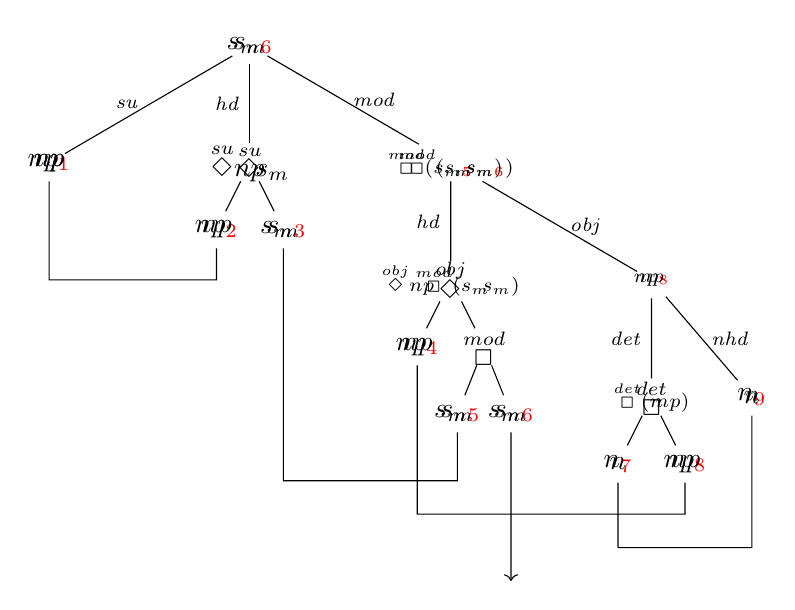
\begin{tikzpicture}[
	every text node part/.style={align=center},
%	every node/.style={transform shape},
	scale=0.85,
	block/.style={rectangle, inner sep=0pt, minimum width=10pt, minimum height=13pt},
	level distance=30pt,
	every leaf node/.style={inner sep=0pt, inner xsep=0pt, outer sep=0pt,distance from root =150pt},
	sibling distance=0.5pt,
	grow=down
	]
	
	\alt<3->{
	% tree repr
	\alt<4->{
		\node[block] (r)			at (7.5, -5.25) 		{$\posat{n}\red{9}$};
		% atoms indexed
		\node[block]	(hn)			at (5.5, -6.25)		{$\negat{n}\red{7}$};
		\node[block]	(hnp)		at (6.5, -6.25)		{$\posat{np}\red{8}$};
		\node[block] (insm1)		at (3.1, -5.5)		{$\negat{s_m}\red{5}$};
		\node[block] (insm2)		at (3.9, -5.5)		{$\posat{s_m}\red{6}$};
		\node[block] (kwakkennp) at (-0.5, -2.75) 	{$\negat{np}\red{2}$};
		\node[block] (kwakkens) 	at (0.5, -2.75) 		{$\posat{s_m}\red{3}$};
		\node[block] (innp)		at (2.5, -4.5)		{$\negat{np}\red{4}$};
		\node[block] (eenden) 	at (-3, -1.75)		{$\posat{np}\red{1}$};
	}{
		\node[block] (r)			at (7.5, -5.25) 		{$\posat{n}$};
		\node[block]	(hn)			at (5.5, -6.25)		{$\negat{n}$};
		\node[block]	(hnp)		at (6.5, -6.25)		{$\posat{np}$};
		\node[block] (insm1)		at (3.1, -5.5)		{$\negat{s_m}$};
		\node[block] (insm2)		at (3.9, -5.5)		{$\posat{s_m}$};
		\node[block] (kwakkennp) at (-0.5, -2.75) 	{$\negat{np}$};
		\node[block] (kwakkens) 	at (0.5, -2.75) 		{$\posat{s_m}$};
		\node[block] (innp)		at (2.5, -4.5)		{$\negat{np}$};
		\node[block] (eenden) 	at (-3, -1.75)		{$\posat{np}$};}
		
	\node[block] (kwakkensu) at (0, -1.75) 		{$\overset{su}{\Diamond}$};
	\draw (kwakkensu) edge (kwakkennp);
	\draw (kwakkensu) edge (kwakkens);

	\node[block] (inobj)		at (3, -3.5)			{$\overset{obj}{\Diamond}$};
	\node[block] (inmod)		at (3.5, -4.5)		{$\overset{mod}{\Box}$};
	\draw (inobj)	edge (innp);
	\draw (inobj)	edge (inmod);
	\draw (inmod)	edge (insm1);
	\draw (inmod)	edge (insm2);
	\node[block]	(h)			at (6, -5.25)		{$\overset{det}{\Box}$};
	\draw (h) edge (hn);
	\draw (h) edge (hnp);
	}{
	% flat repr
	\node[block] (eenden) 	at (-3, -1.75)		{$np$};
	\node[block] (kwakken) 	at (0, -1.75) 		{${\overset{su}{\Diamond}}np\li {s_m}$};
	\node[block] (in)		at (3, -3.5) 		{\type{\overset{obj}{\Diamond}np\!\li\!\!\overset{mod}{\Box}({s_m}\li {s_m}) }{black}};
	\node[block] (h)			at (6, -5.25) 		{\type{\overset{det}{\Box}(n\li np)}{black}};
	\node[block] (r)			at (7.5, -5.25) 		{\type{n}{black}};}

	\alt<7->{	
	\node[block] (smain) 	at (0, 0) 			{$s_m\red{6}$};	
	\draw (kwakkens) -- (0.5, -6.5) -- (3.1, -6.5) -- (insm1);
	\draw (insm2)	edge[->] (3.9, -8);
	}{
	\node[block] (smain) 	at (0, 0) 			{$s_m$};	
	}
	
	\alt<6->{
	\node[block] (ihr)		at (3, -1.75) 		{\type{\overset{mod}{\Box}(s_m\red{5}\li s_m\red{6})}{black}};
	\draw (hnp) -- (6.5, -7) -- (2.5, -7) -- (innp);
	}{
	\node[block] (ihr)		at (3, -1.75) 		{\type{\overset{mod}{\Box}(s_m\li s_m)}{black}};}

	\alt<5->{
	\node[block] (hr)		at (6, -3.5) 		{\type{np\red{8}}{black}};
	\draw (hn) -- (5.5, -7.5) -- (7.5, -7.5) -- (r);
	\draw (eenden) -- (-3, -3.5) -- (-0.5, -3.5) -- (kwakkennp);
	}{	
	\node[block] (hr)		at (6, -3.5) 		{\type{np}{black}};}

	
	\draw (smain) 	edge[-]		node[left] 	{\etext{su}} 	(eenden);
	\draw (smain) 	edge[-]		node[left] 	{\etext{hd}} 	(kwakken);
	\draw (smain) 	edge[-]		node[right] {\etext{mod}} 	(ihr);
	
	\draw (ihr)	 	edge[-]		node[left] 	{\etext{hd}} 		(in);
	\draw (ihr)	 	edge[-]		node[right] {\etext{obj}} 		(hr);
	
	\draw(hr)		edge[-]		node[left] 	{\etext{det}}		(h);
	\draw(hr)		edge[-]		node[right] {\etext{nhd}}		(r);
	\end{tikzpicture}
	\vfill
	
	\visible<1>{given a typed graph:\\}
	\alt<2>{(1) convert types to binary trees and assign polarities}
	{\alt<3>{(2) assign identifying indices}{
	\alt<8>{the resulting structure is a \textit{proof net}}{
	\alt<4->{(3) traverse upwards, identifying pos/neg atoms and propagating indices\\
	}}{}}}
	
%	\scriptsize
%		\begin{itemize}
%			\item init an empty map $\mathbb{N} \to \mathbb{N}$
%			\visible<2->{
%			\item assign a unique identifying index to each atom in the graph's fringe}
%			\visible<4->{
%			\item traversing up, identify argument indices with siblings and result indices with parents}
%		\end{itemize}
%	\vfill
%	\end{minipage}
%	\[
%		\visible<5->{6:8
%		\visible<6->{,~3:7}
%		\visible<7->{,~2:1,~3:4}
%		}
%	\]
\end{frame}

	
%\begin{frame}{From graphs to proofs}	
%	\small
%	\begin{tikzpicture}
%	\node (eenden)			at (0, 0)		{\proofspace{\text{eenden}}};
%	\node (eenden_np)		at (0, 2em)		{$\posat{np}_1$};
%	
%	\node (kwakken)			at (5em, 0em)	{\proofspace{\text{kwakken}}};
%	\node (kwakken_su)		at (5em, 2em)	{$\proofspace{\Diamond^{su}}$};
%	\node (kwakken_np)		at (3em, 5em)	{$\negat{np}_2$};
%	\node (kwannen_s)		at (7em, 5em)	{$\posat{s_m}_3$};
%	\end{tikzpicture}
%\end{frame}
%
\end{document}